%!TEX root = report.tex

\todo[inline]{Geen grounding -> ballon effect -> add grounding springs. Compare results.}

\todo[inline]{Compare different methods of breaking}

\todo[inline]{Compare different numbers of springs to break per step}


\begin{figure*}
	\centering
	\begin{subfigure}{0.16\textwidth}
		\centering
		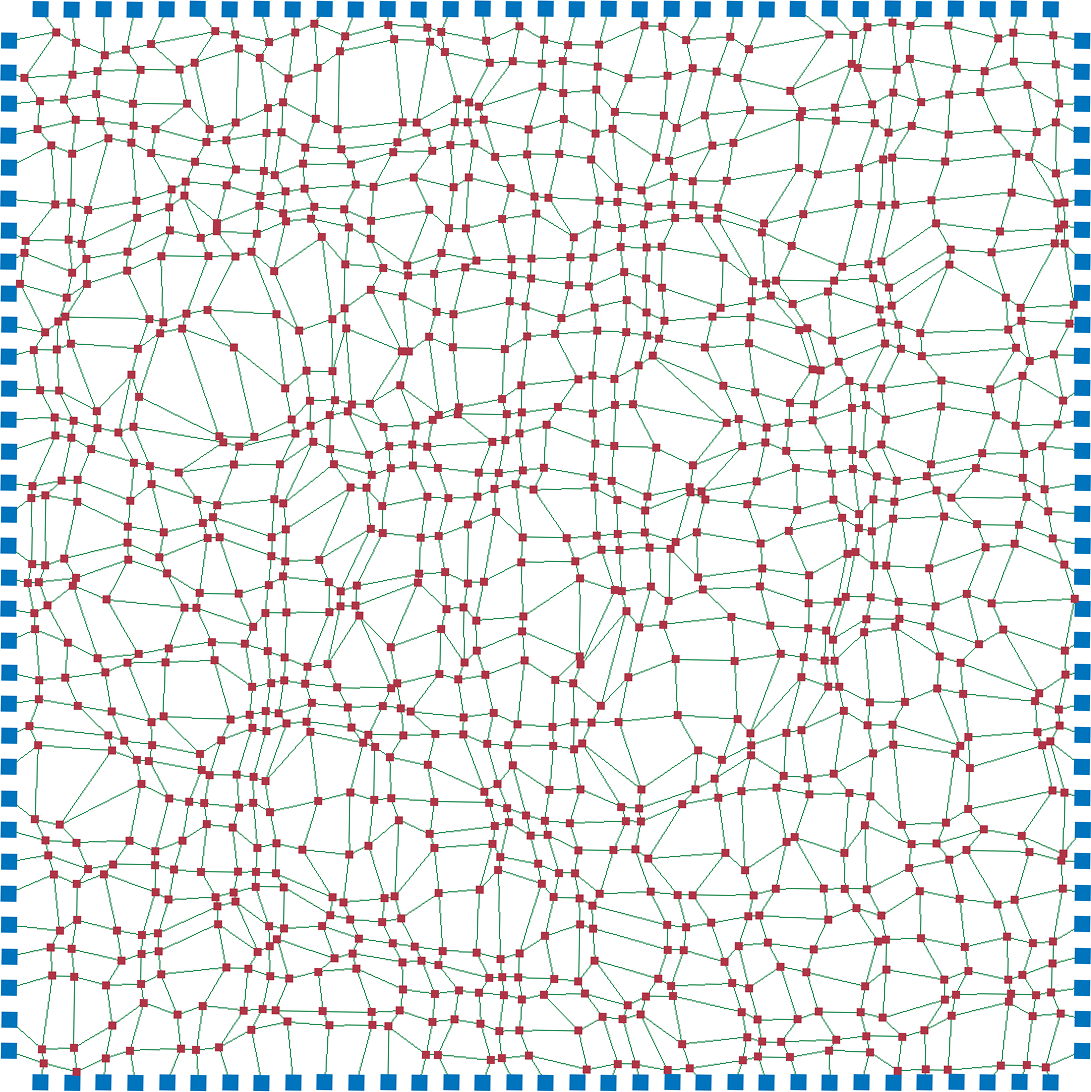
\includegraphics[
			width=\textwidth, 
			height=\textwidth, 
			keepaspectratio=true]
		{./img/results/1200_0_1_highest_97_step_0}
		\caption{Step 0}
		\label{fig:experiment:highestStrain:0}
	\end{subfigure}
	\begin{subfigure}{0.16\textwidth}
		\centering
		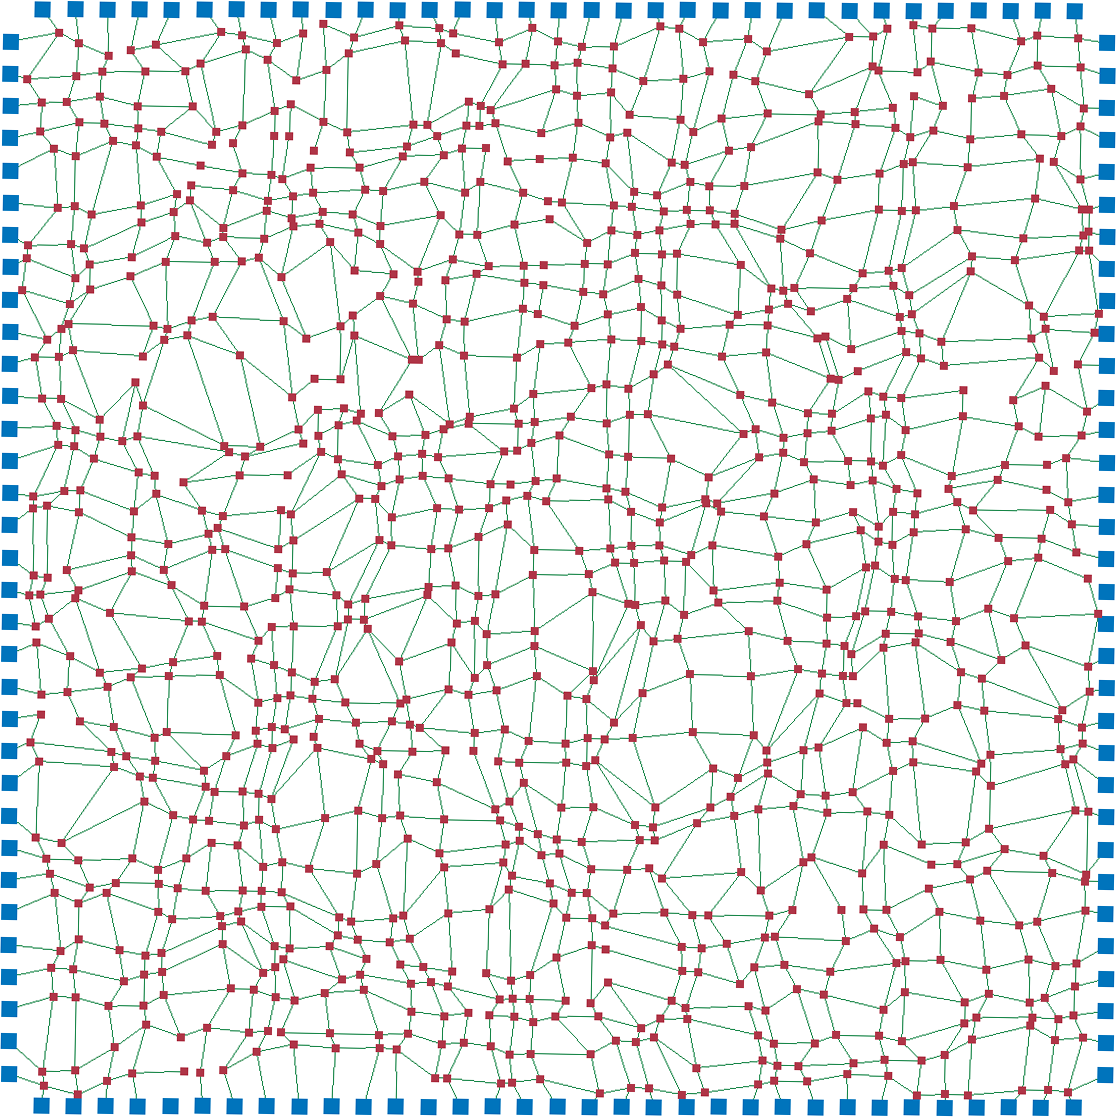
\includegraphics[
			width=\textwidth, 
			height=\textwidth, 
			keepaspectratio=true]
		{./img/results/1200_0_1_highest_97_step_1}
		\caption{Step 1}
		\label{fig:experiment:highestStrain:1}
	\end{subfigure}	
	\begin{subfigure}{0.16\textwidth}
		\centering
		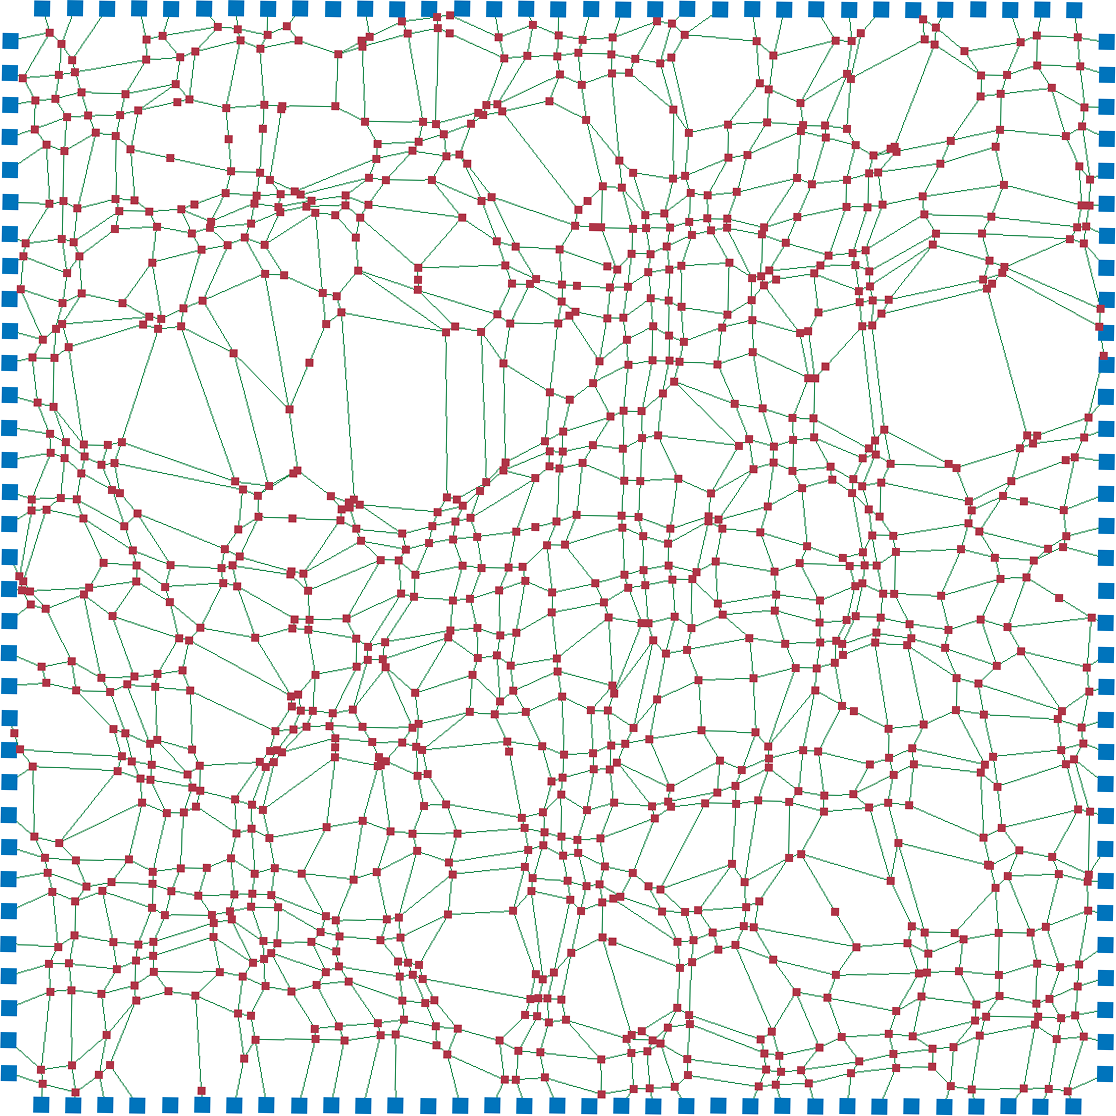
\includegraphics[
			width=\textwidth, 
			height=\textwidth, 
			keepaspectratio=true]
		{./img/results/1200_0_1_highest_97_step_2}
		\caption{Step 2}
		\label{fig:experiment:highestStrain:2}
	\end{subfigure}		
	\begin{subfigure}{0.16\textwidth}
		\centering
		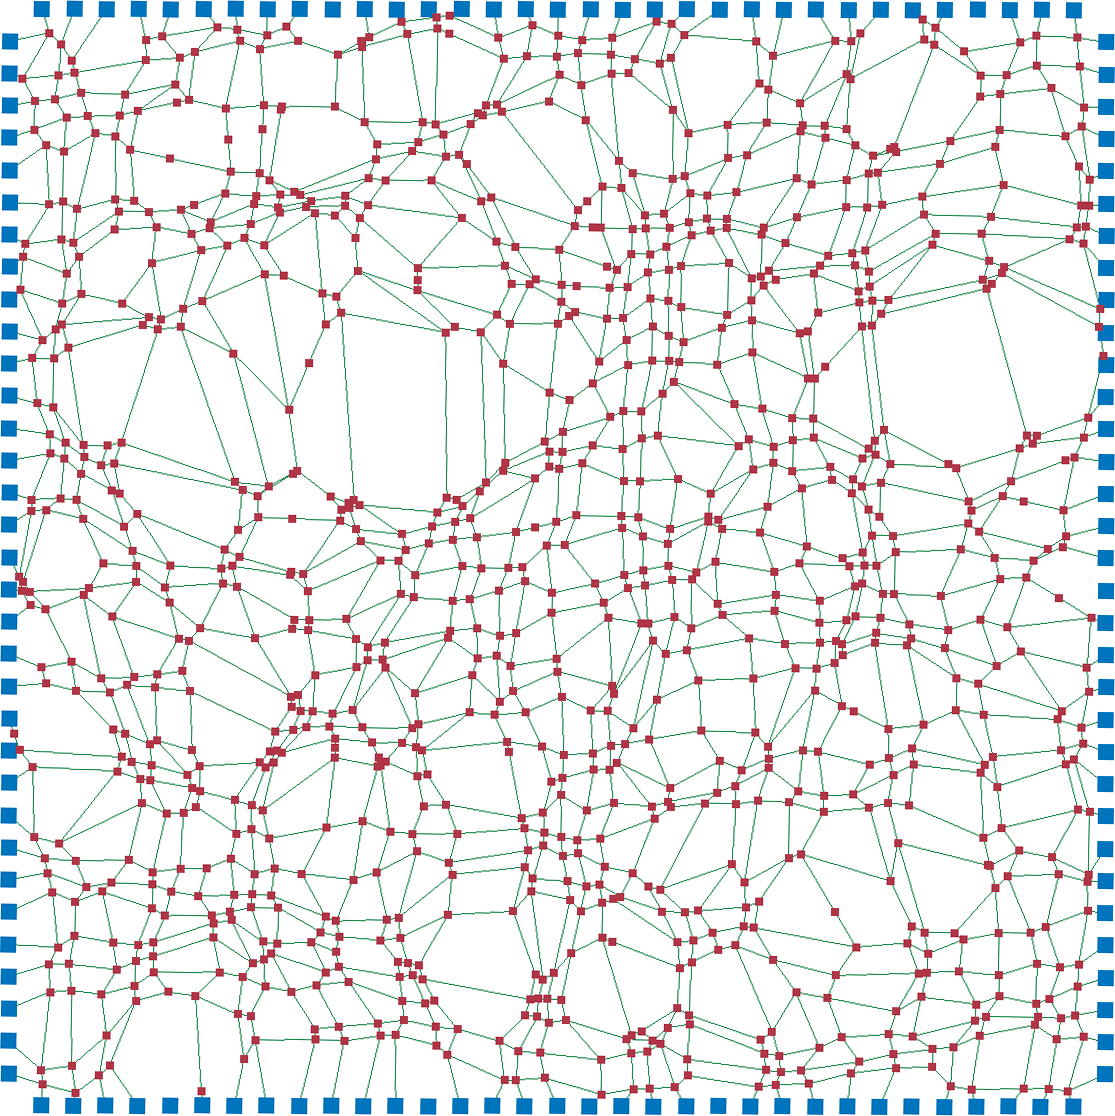
\includegraphics[
			width=\textwidth, 
			height=\textwidth, 
			keepaspectratio=true]
		{./img/results/1200_0_1_highest_97_step_3}
		\caption{Step 3}
		\label{fig:experiment:highestStrain:3}
	\end{subfigure}			
	\begin{subfigure}{0.16\textwidth}
		\centering
		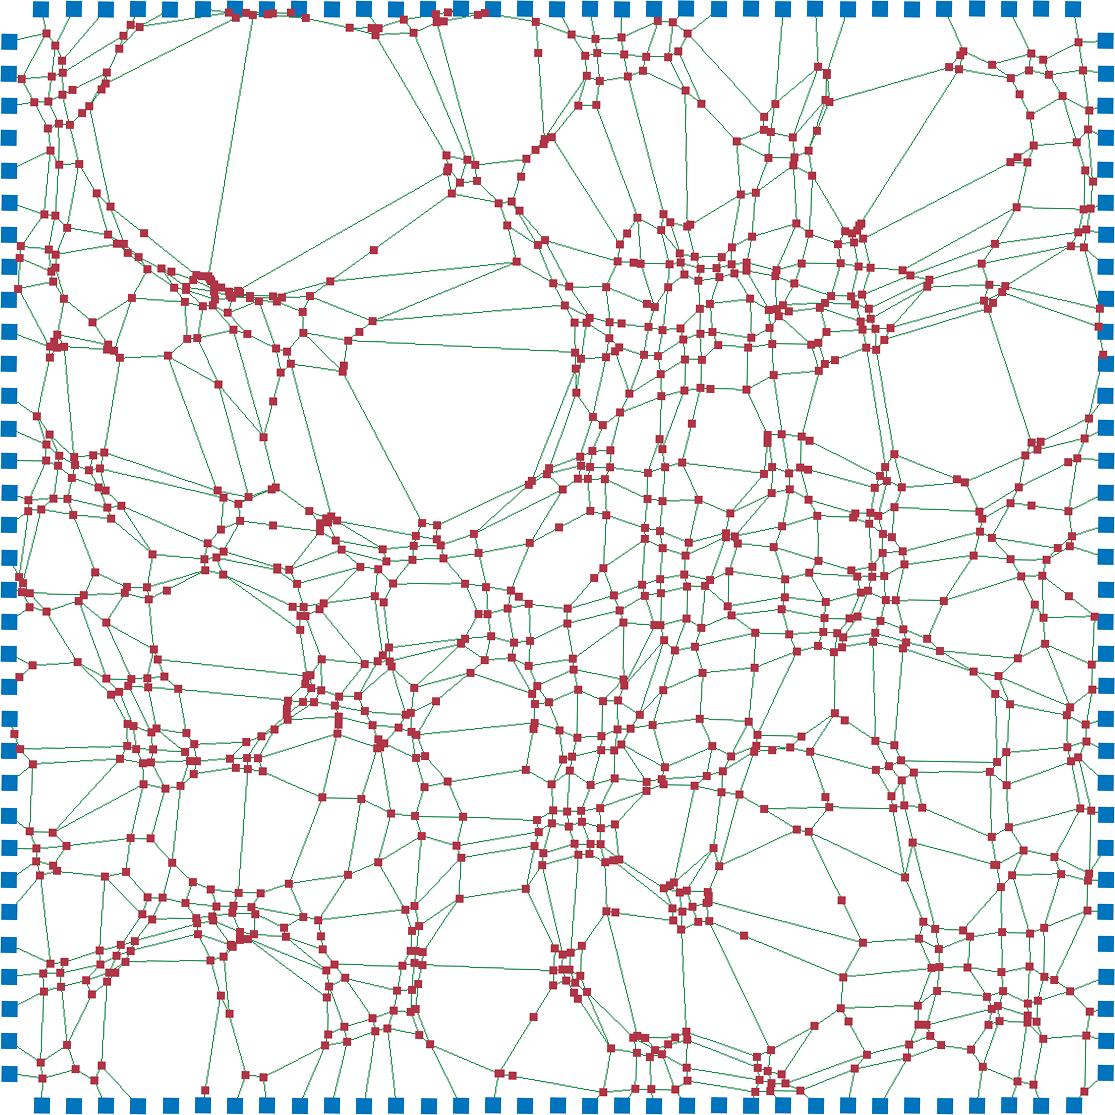
\includegraphics[
			width=\textwidth, 
			height=\textwidth, 
			keepaspectratio=true]
		{./img/results/1200_0_1_highest_97_step_4}
		\caption{Step 4}
		\label{fig:experiment:highestStrain:4}
	\end{subfigure}				
	\begin{subfigure}{0.16\textwidth}
		\centering
		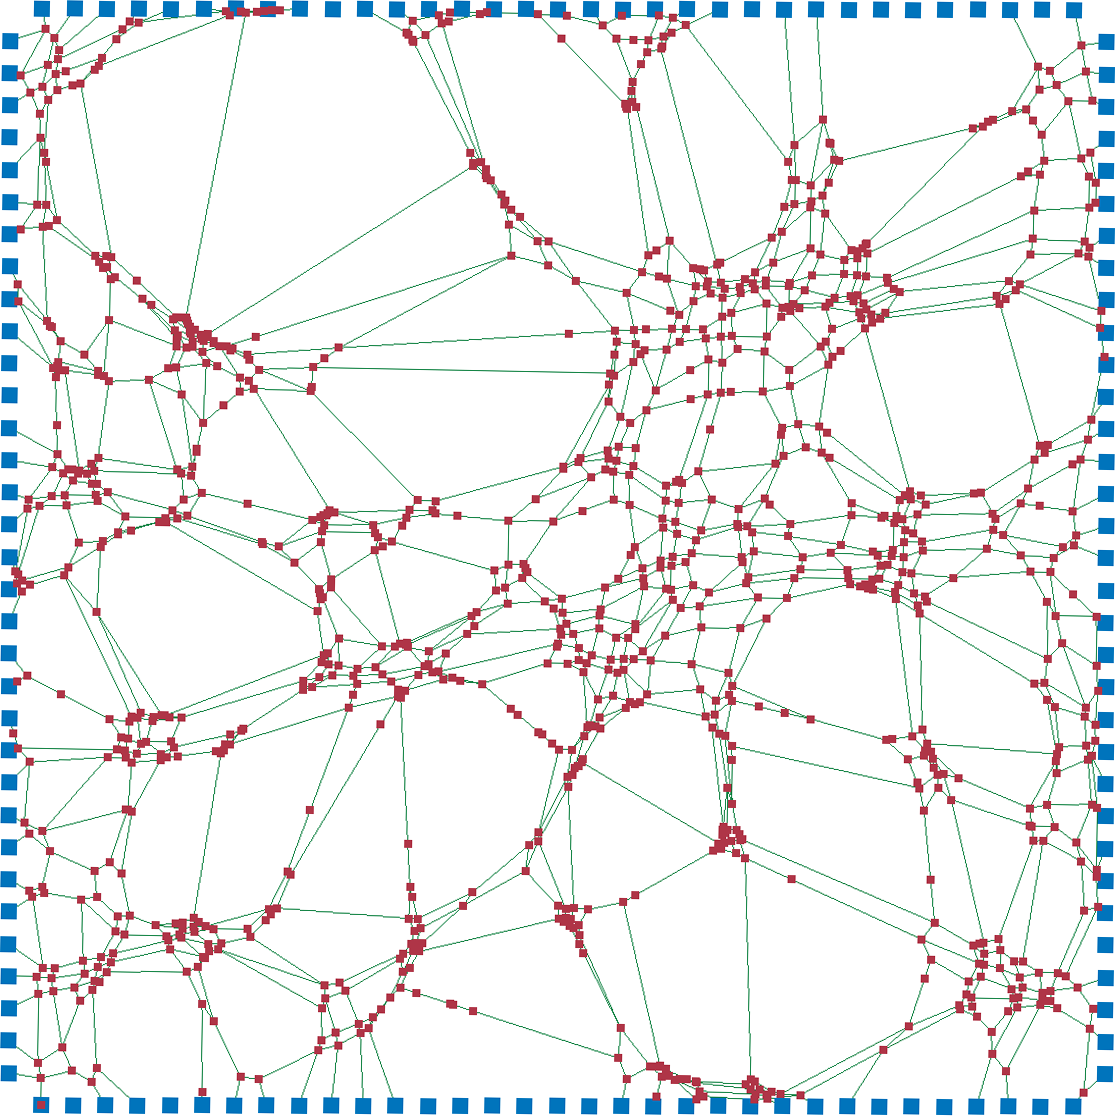
\includegraphics[
			width=\textwidth, 
			height=\textwidth, 
			keepaspectratio=true]
		{./img/results/1200_0_1_highest_97_step_5}
		\caption{Step 5}
		\label{fig:experiment:highestStrain:5}
	\end{subfigure}
	\begin{subfigure}{0.16\textwidth}
		\centering
		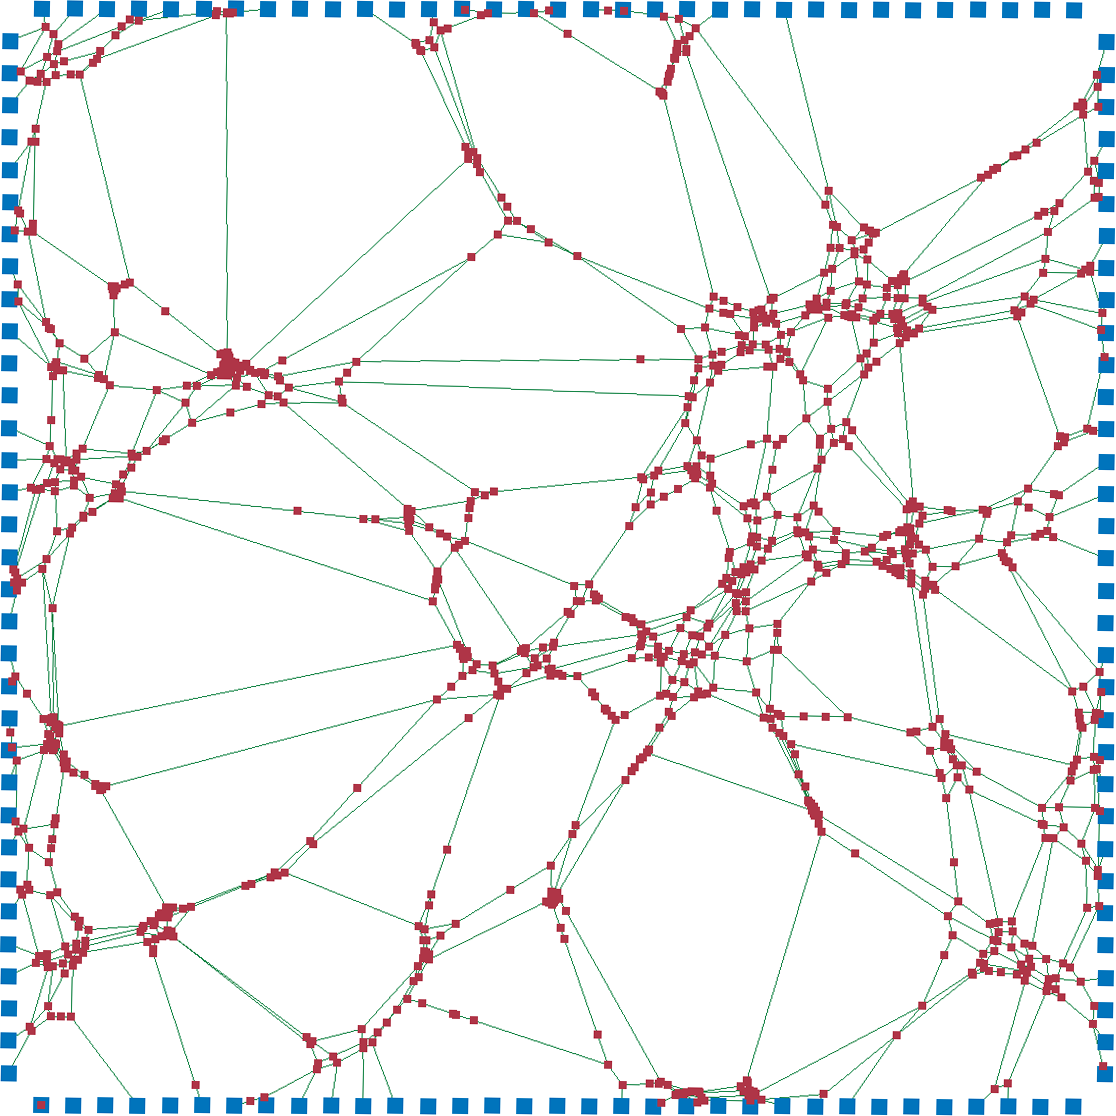
\includegraphics[
			width=\textwidth, 
			height=\textwidth, 
			keepaspectratio=true]
		{./img/results/1200_0_1_highest_97_step_6}
		\caption{Step 6}
		\label{fig:experiment:highestStrain:6}
	\end{subfigure}	
	\begin{subfigure}{0.16\textwidth}
		\centering
		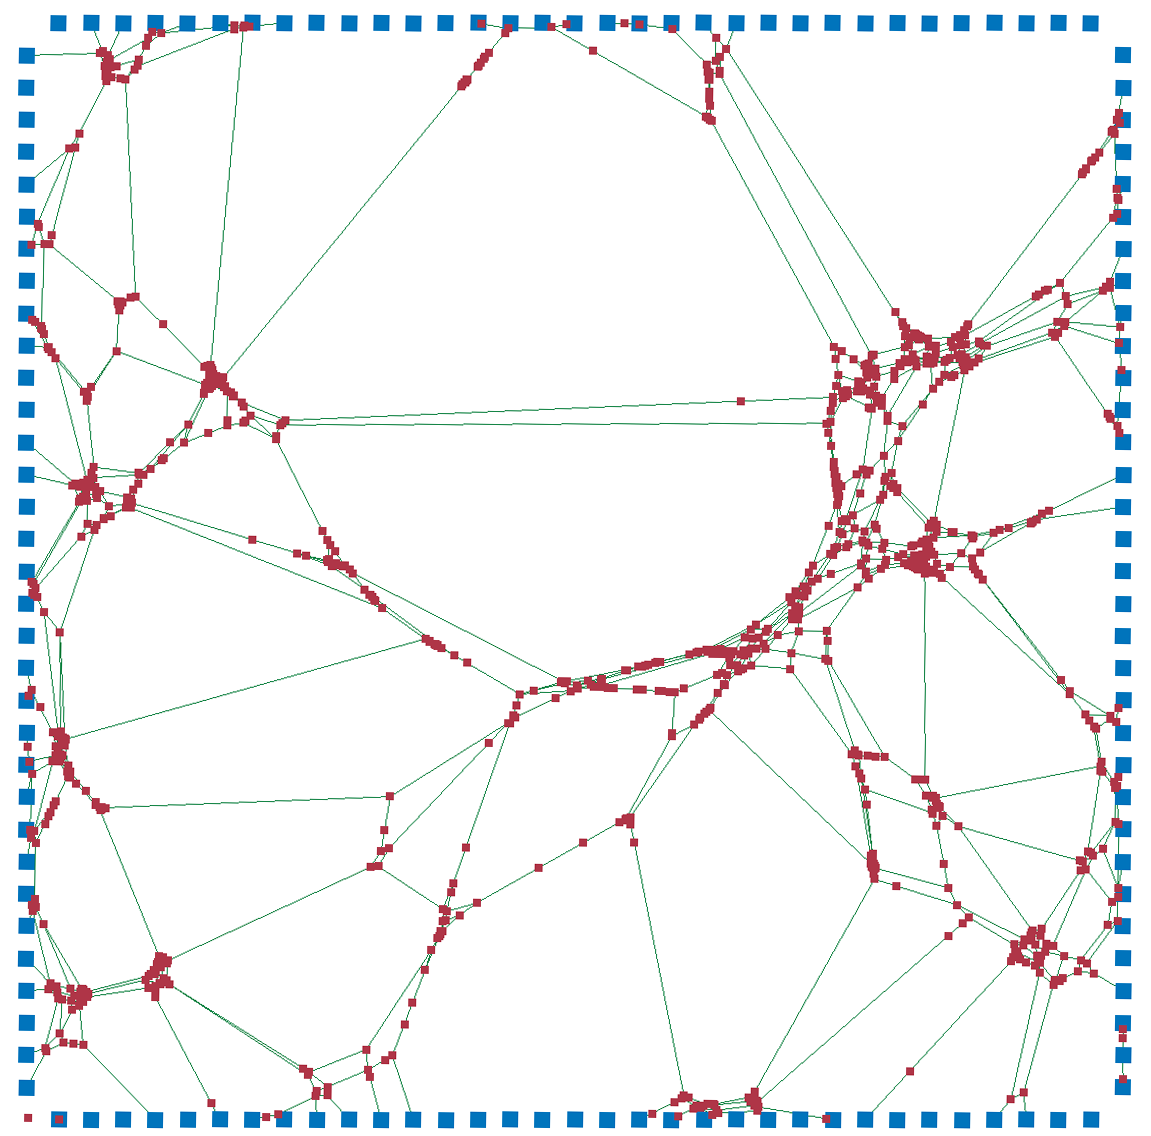
\includegraphics[
			width=\textwidth, 
			height=\textwidth, 
			keepaspectratio=true]
		{./img/results/1200_0_1_highest_97_step_7}
		\caption{Step 7}
		\label{fig:experiment:highestStrain:7}
	\end{subfigure}		
	\begin{subfigure}{0.16\textwidth}
		\centering
		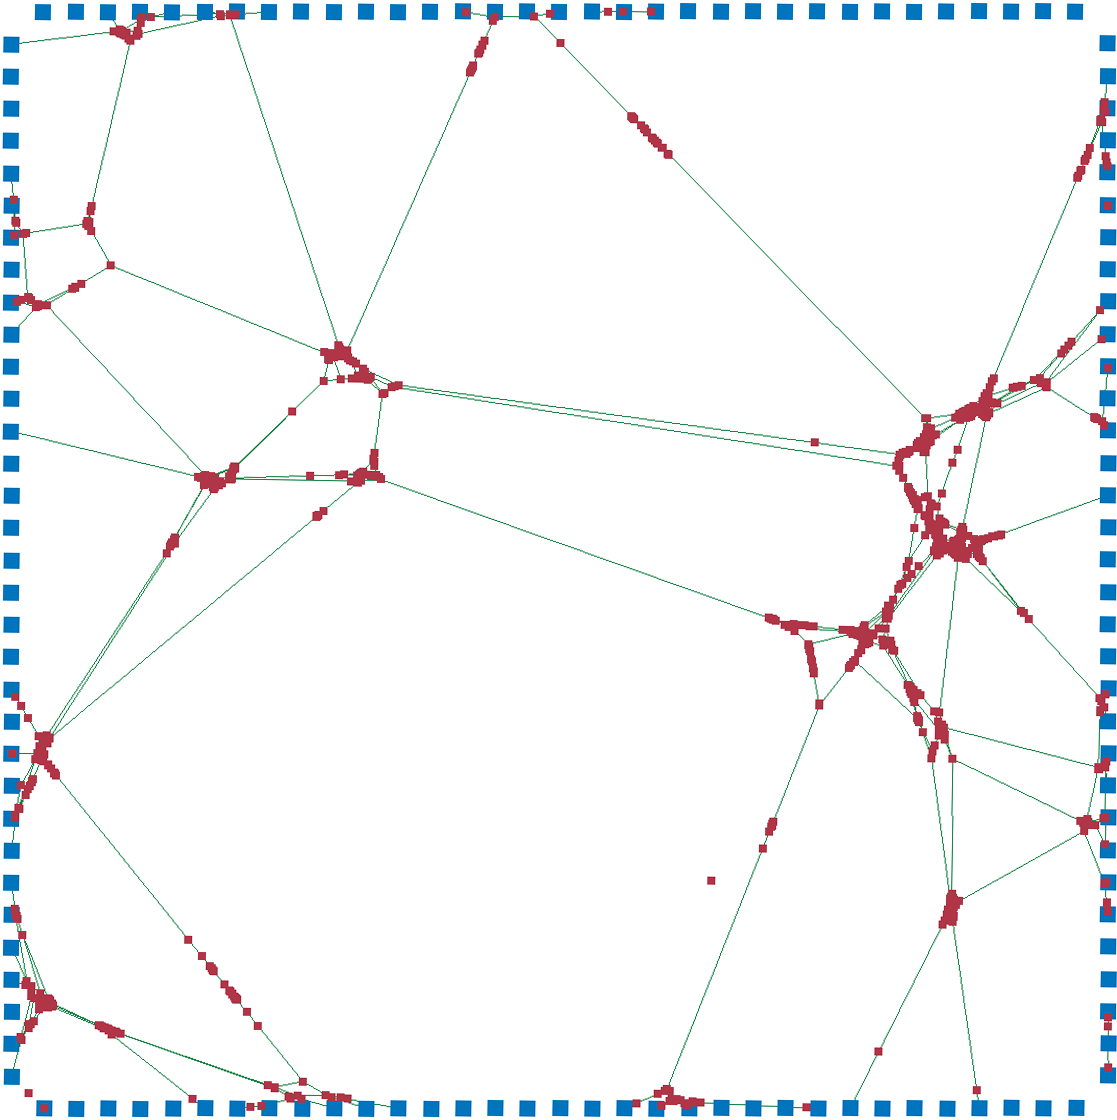
\includegraphics[
			width=\textwidth, 
			height=\textwidth, 
			keepaspectratio=true]
		{./img/results/1200_0_1_highest_97_step_8}
		\caption{Step 8}
		\label{fig:experiment:highestStrain:8}
	\end{subfigure}			
	\begin{subfigure}{0.16\textwidth}
		\centering
		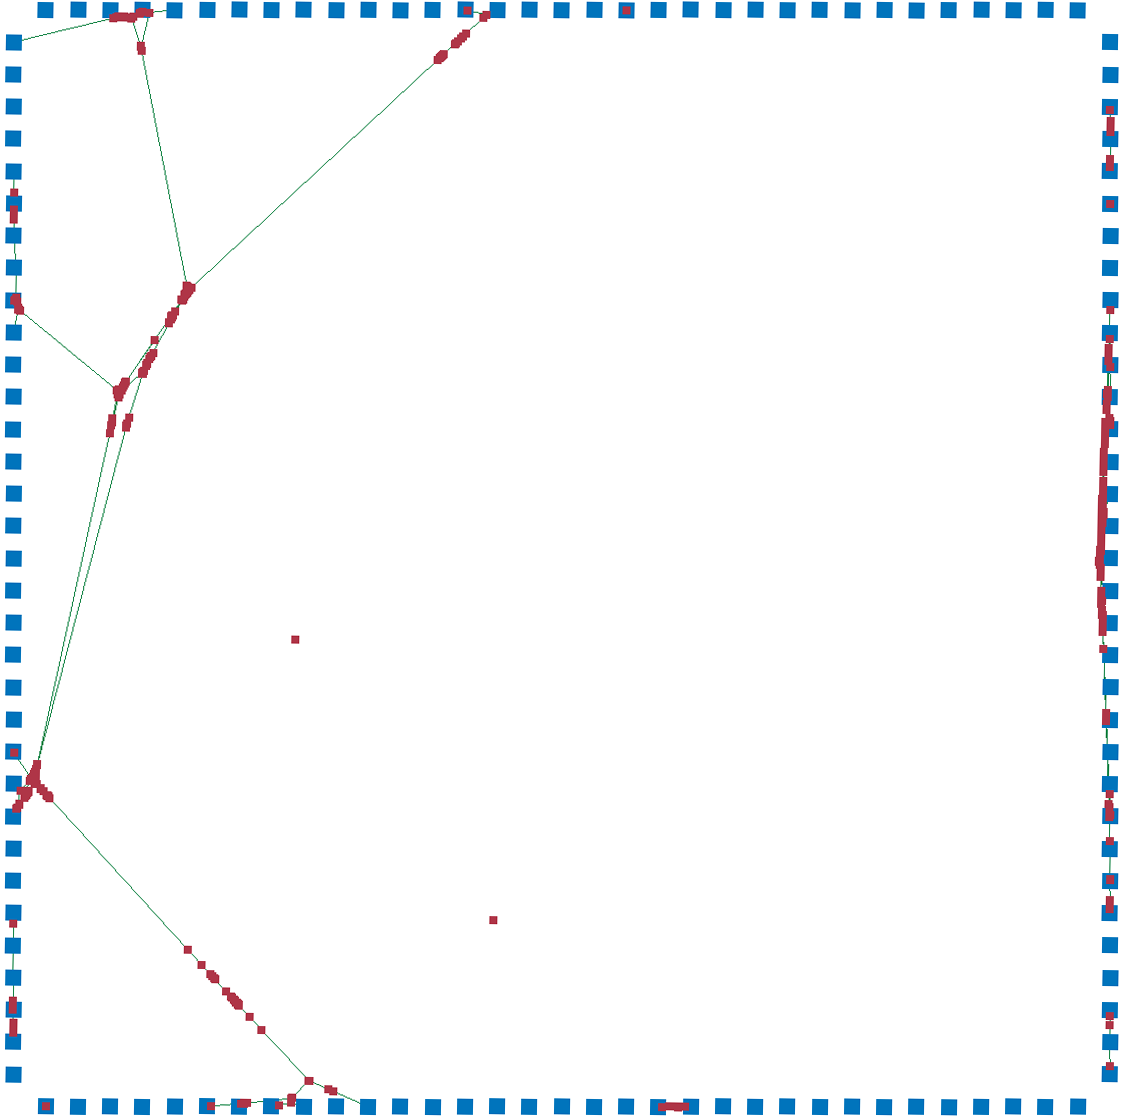
\includegraphics[
			width=\textwidth, 
			height=\textwidth, 
			keepaspectratio=true]
		{./img/results/1200_0_1_highest_97_step_9}
		\caption{Step 9}
		\label{fig:experiment:highestStrain:9}
	\end{subfigure}					
	\begin{subfigure}{0.16\textwidth}
		\centering
		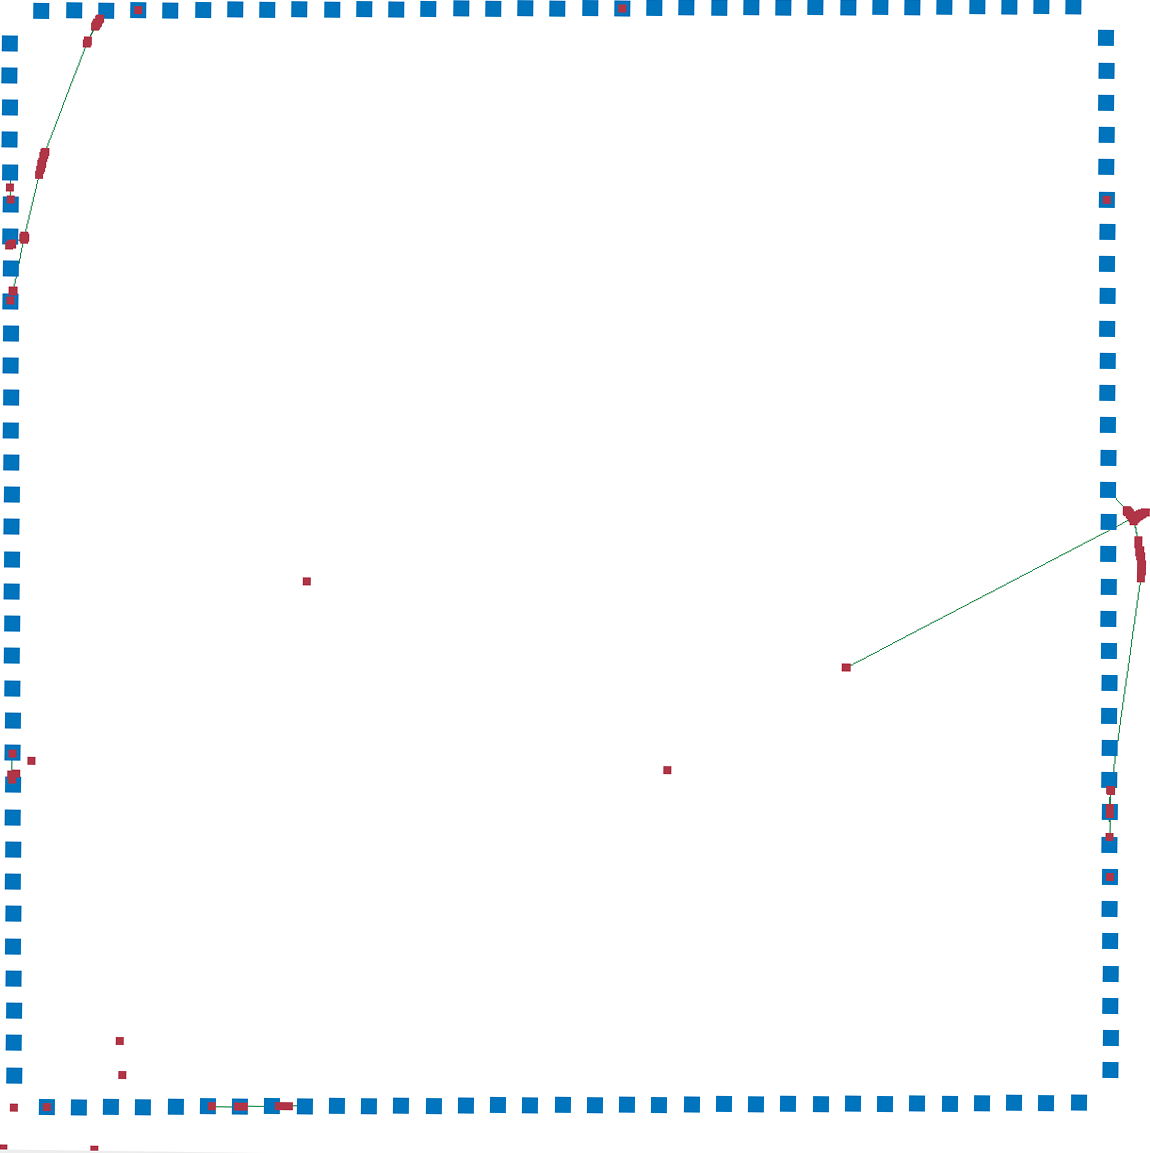
\includegraphics[
			width=\textwidth, 
			height=\textwidth, 
			keepaspectratio=true]
		{./img/results/1200_0_1_highest_97_step_10}
		\caption{Step 10}
		\label{fig:experiment:highestStrain:10}
	\end{subfigure}			
	\begin{subfigure}{0.16\textwidth}
		\centering
		
\includegraphics[
			width=\textwidth, 
			height=\textwidth, 
			keepaspectratio=true]
		{./img/results/1200_0_1_highest_97_step_11}
		\caption{Step 11}
		\label{fig:experiment:highestStrain:11}
	\end{subfigure}						
	\caption{Several steps of the breaking of springs, where the 97 springs with the highest strain were broken. The grid had 1200 particles, the spring constants were sampled from a normal distribution with mean 0.0 and standard deviation 1.0. Step 0 is a stabilization of the initial grid, presented in \cref{fig:implementation:stabilizedInitial}, the following steps are the stabilization and breaking steps of the algorithm.}
	\label{fig:experiment:highestStrain}
\end{figure*}